
\documentclass{beamer}
\usetheme{Electromagnetism}
\usepackage{Electromagnetism}
\usetikzlibrary{intersections}
\graphicspath{{pictures/}}
% -------------------------------------- Grid
%-------------------------------------------------------
\makeatletter
\def\grd@save@target#1{%
  \def\grd@target{#1}}
\def\grd@save@start#1{%
  \def\grd@start{#1}}
\tikzset{
  grid with coordinates/.style={
    to path={%
      \pgfextra{%
        \edef\grd@@target{(\tikztotarget)}%
        \tikz@scan@one@point\grd@save@target\grd@@target\relax
        \edef\grd@@start{(\tikztostart)}%
        \tikz@scan@one@point\grd@save@start\grd@@start\relax
        \draw[minor help lines] (\tikztostart) grid (\tikztotarget);
        \draw[major help lines] (\tikztostart) grid (\tikztotarget);
        \grd@start
        \pgfmathsetmacro{\grd@xa}{\the\pgf@x/1cm}
        \pgfmathsetmacro{\grd@ya}{\the\pgf@y/1cm}
        \grd@target
        \pgfmathsetmacro{\grd@xb}{\the\pgf@x/1cm}
        \pgfmathsetmacro{\grd@yb}{\the\pgf@y/1cm}
        \pgfmathsetmacro{\grd@xc}{\grd@xa + \pgfkeysvalueof{/tikz/grid with coordinates/major step}}
        \pgfmathsetmacro{\grd@yc}{\grd@ya + \pgfkeysvalueof{/tikz/grid with coordinates/major step}}
        \foreach \x in {\grd@xa,\grd@xc,...,\grd@xb}
        \node[anchor=north] at (\x,\grd@ya) {\pgfmathprintnumber{\x}};
        \foreach \y in {\grd@ya,\grd@yc,...,\grd@yb}
        \node[anchor=east] at (\grd@xa,\y) {\pgfmathprintnumber{\y}};
      }
    }
  },
  minor help lines/.style={
    help lines,
    step=\pgfkeysvalueof{/tikz/grid with coordinates/minor step}
  },
  major help lines/.style={
    help lines,
    line width= 0.5pt,
    step=\pgfkeysvalueof{/tikz/grid with coordinates/major step}
  },
  grid with coordinates/.cd,
  minor step/.initial=.2,
  major step/.initial=1,
  major line width/.initial=2pt,
}
\makeatother
\usepackage{cancel}
\begin{document}


% ============================== Слайд ## ===================================
\begin{frame}{}{}
	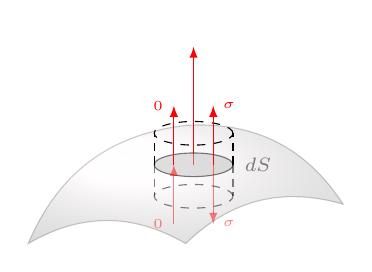
\begin{tikzpicture}[>=latex, every node/.style={font=\scriptsize},
			transform shape]
        \pgfmathsetmacro\h{0.4}
        \pgfmathsetmacro\r{0.5}
		\begin{scope}[opacity=0.2]
			\draw[ball color=red!5] (0,0) to[bend left] ++(2,1.5)  to[bend left] ++(2,-1)
			to[bend right]
			++(-2, -0.5)  to[bend
				right] cycle;

		\end{scope}

        \pgfmathsetmacro\x{2.1}
        \pgfmathsetmacro\y{1.0}
        \coordinate (A)  at (\x,          \y);
        \coordinate (A1) at ({\x - \r},   \y);
        \coordinate (A2) at ({\x + \r},   \y);
        \coordinate (E0) at ({\x - \r/2}, \y);
        \coordinate (Es) at ({\x + \r/2}, \y);

		\draw[->, red]  (A) -- ++(90:1.5) coordinate (B)
		node[above] {$\Efield$};

		\draw[fill=gray!50, opacity=0.5] (A) circle[x radius =\r, y radius= 0.15] node[right=15pt]
		{$dS$};
		\draw[dashed] (A) ++(90:\h) circle[x radius =\r, y radius= 0.15];

		\draw[densely dashed] (A1) -- ++(90:\h);
		\draw[densely dashed] (A2) -- ++(90:\h);

        \draw[->, red] (Es) -- ++(0,+0.75) node[right] {$\Efield_{\sigma}$};
        \draw[->, red] (E0) -- ++(0,+0.75) node[left] {$\Efield_{0}$};

        \begin{scope}[opacity=0.5]
            \draw[densely dashed] (A1) -- ++(90:-\h);
    		\draw[densely dashed] (A2) -- ++(90:-\h);
            \draw[dashed] (A) ++(90:-\h) circle[x radius =\r, y radius= 0.15];

            \draw[->, red] (Es) -- ++(0,-0.75) node[right] {$\Efield_{\sigma}$};
            \draw[<-, red] (E0) -- ++(0,-0.75) node[left] {$\Efield_{0}$};
        \end{scope}

	\end{tikzpicture}
\end{frame}
% ===========================================================================





\end{document}